
    \Cref{chapter:theory} derived an approach for constraint programming on
    Static Single Assignment (SSA) compiler intermediate representation.
    This chapter develops a novel domain-specific constraint programming
    language based on that methodology and presents an implementation within the
    production-quality LLVM compiler infrastructure.

    In the first sections, the design of the Compiler Analysis
    Description Language (CAnDL) is motivated as an approach for simplifying
    the implementation of LLVM transformation passes.
    Optimising compilers have to use elaborate program transformations to
    exploit increasingly complex hardware.
    Implementing the required analysis functionality for such optimisations to
    be safely applied is a time-consuming and error-prone activity.
    This is a barrier to the rapid prototyping and evaluation of innovative new
    compiler optimisations.
    CAnDL automatically generates such compiler analysis functionality from
    constraint specifications.

    The individual language constructs are introduced with their syntax and
    functionality in the central section of this chapter.
    The first introduced language features directly expose parts of the
    underlying SSA model from \Cref{chapter:theory}.
    Building on that, CAnDL provides higher-level constructs that allow for
    modularity in specifications and the reduction of repetitive constraints.
    Using these higher-level constructs, a collection of CAnDL specifications
    of standard compiler concepts is introduced as the CAnDL standard library.
    This collection of common building blocks includes single-entry single-exit
    regions, loops, and array-based memory accesses.

    Finally, several case studies are presented for the experimental evaluation
    of CAnDL.
    They show that CAnDL scales to a wide range of compiler analysis tasks.
    These tasks range from the detection of peephole optimisation opportunities,
    over graphics shader optimisations, to fully capturing Static Control Parts
    (SCoPs) for polyhedral code analysis.
    All of them can be expressed more succinctly in CAnDL than with previous
    approaches.

\section{Introduction}

    Compilers are intricate pieces of software responsible for the generation of
    efficient code.
    They transform input source code through several compilation stages,
    resulting in a binary program.
    In order to generate fast programs, state-of-the-art compilers rely on an
    elaborate middle end.
    At this stage, the user code is typically expressed in an SSA intermediate
    representation, and improved by successively applying a wide range of
    optimisations.

    Most compiler optimisations require two steps:
    analysis and transformation.
    First, analysis routines find sections in user programs that enable the
    application of specific transformations.
    They further verify the necessary conditions to ensure the transformation
    can be applied legally without changing the program semantics.
    It is crucial that optimisations retain the semantics of the original
    program, as otherwise the resulting binary might be corrupted.
    Transformations are then applied to the analysis results in a second step.
    This often involves heuristic cost models to gauge the effect on runtime,
    code size, and other metrics.

    The complexity of the necessary analysis is an impediment to
    the implementation of new compiler passes, preventing the rapid
    prototyping of new ideas.
    For example, simple peephole optimisations in the LLVM ``{\tt instcombine}''
    pass require approximately 30000 lines of C++ code, despite the
    transformations being simple.
    \citet{Menendez:2017:ADP:3062341.3062372} showed that ``{\tt instcombine}''
    is an important source of bugs, and bugs in the middle end of a compiler are
    particularly pernicious \citep{Yang:2011:FUB:1993316.1993532}.
    They tamper with the user programs but can remain unnoticed and often only
    trigger in corner cases.
    Ideally, there would be a simpler way of implementing such analysis that
    reduces boilerplate code and opens the way for new compiler innovation.

    This chapter presents the Compiler Analysis Description Language (CAnDL), a
    domain-specific language for compiler analysis.
    It is a constraint programming language, operating on the SSA intermediate
    representation of the LLVM compiler infrastructure (LLVM IR).
    Instead of writing compiler analysis code inside the main codebase of the
    compiler infrastructure, it lets compiler writers specify optimisation
    functionality external to the main C++ codebase.
    The CAnDL compiler then generates C++ functions that implement LLVM analysis
    passes, and are linked together with the Clang compiler binary.
    The formulation of optimising transformations in CAnDL is faster, simpler
    and less error-prone than writing them in C++.
    The language has a strong emphasis on modularity, which facilitates
    debugging and the formulation of highly readable code.

    CAnDL is based on the constraint programming methodology introduced in
    \Cref{chapter:theory}.
    It uses a solver that is integrated into the LLVM codebase.
    CAnDL is developed as a complete programming language, with a full parser
    and code generator.
    The system is evaluated on a range of use cases from
    different domains, including standard LLVM optimisation passes,
    custom optimisations for graphics shader programs, and the detection of
    Static Control Parts (SCoPs) \citep{Lengauer2012Polly} for polyhedral
    program transformations \citep{Karp:1967:OCU:321406.321418}.

\section{Motivating Example}

\begin{figure}[b]
\centering
\begin{minipage}[t]{0.68\textwidth}
\begin{lstlisting}[language=CAnDL,label={fig:candlspec},caption=
   {The left side of \Cref{fig:root} as specified in CAnDL}]
Constraint SqrtOfSquare
( opcode{sqrt_call} = call
∧ {sqrt_fn} = {sqrt_call}.args[0]
∧ function_name{sqrt_fn} = sqrt
∧ {square} = {sqrt_call}.args[1]
∧ opcode{square} = fmul
∧ {a} = {square}.args[0]
∧ {a} = {square}.args[1])
End
\end{lstlisting}
\end{minipage}
\end{figure}

    For an example of the CAnDL workflow, consider \Cref{fig:root}.
    This basic algebraic equation can be interpreted as a recipe for a compiler
    optimisation:
    Assuming an environment without the particularities of floating-point
    arithmetic (i.e.\ assuming the \texttt{-ffast-math} flag is active), the
    compiler could use this equality to eliminate some square root invocations
    in user code.
    This is desirable, as the square root has to be approximated with relatively
    expensive numerical methods, whereas computing the absolute value is
    computationally cheap.
    \begin{align}
    \label{fig:root}
    \forall a\in \mathbb{R}\colon\ \sqrt{a*a}=|a|
    \end{align}

    The compiler should use the equation left-to-right.
    It should analyse the user code in order to find segments that correspond to
    the left side of the equation and then transform all those occurrences
    analogous to the right side of the equation.
    The compiler, therefore, must detect $\sqrt{a*a}$ in the LLVM IR code and
    replace it with calls to the ``\texttt{abs}'' function.
    The generation of the new function call is trivial, but the detection of
    even this simple pattern requires some care when implemented manually in
    a sophisticated codebase such as LLVM.

    The traditional approach in the Clang compiler is to integrate such
    optimisations into the previously mentioned ``\texttt{instcombine}'' pass.
    which already applies an extensive collection of peephole optimisations.
    However, this code makes heavy use of raw pointers and dynamic type casts,
    spans ${\sim}30000$ lines, and has been identified as a frequent source of
    bugs in
    \citet{Menendez:2017:ADP:3062341.3062372,Yang:2011:FUB:1993316.1993532}.
    This is impractical and an impediment to compiler development.

    Instead, CAnDL allows a declarative description of the analysis problem.
    It is easier to follow, has no interaction with other optimisations and
    is concise, as presented in \Cref{fig:candlspec}.
    The first line of the program assigns a name to the specification, which is
    then defined by the interaction of seven {\em atomic constraint}s.
    These individual statements must simultaneously hold on the values of
    ``\texttt{sqrt\_call}'', ``\texttt{sqrt\_fn}'', ``\texttt{square}'' and
    ``\texttt{a}''.
    Lines 2--8 each stipulate one of these constraints, and they are joined
    together with logical conjunctions ``$\land$''.

    The CAnDL compiler translates the declarative program into a C++ function,
    which is then used for the analysis step in an LLVM optimisation pass.
    This is demonstrated in \Cref{fig:candlexample}, which shows the application
    of the analysis function generated from the CAnDL specification in
    \Cref{fig:candlspec} to a user program.
    The input program ({\bf a}) is a simple C function that calls the
    ``\texttt{sqrt}'' function twice with squares of floating-point values.
    This is translated using the Clang compiler into LLVM IR code ({\bf b}),
    using standard optimisation passes during the compilation.
    The expression from the user program is here represented as a list of
    individual instructions and register assignments, with the occurrences
    of ``\texttt{SqrtOfSquare}'' clearly visible: the two ``\texttt{fmul}''
    instructions (lines 4 and 6) compute squares via a floating-point
    multiplication, and these are then used as arguments to ``\texttt{sqrt}''
    function invocations (lines 5 and 7).

    The optimised LLVM IR ({\bf b}) is used as the input to the generated
    analysis function, which detects two optimisation opportunities.
    These are identified as the first ({\bf c}) and second ({\bf d}) solution
    of the constraint problem.
    Each of the solutions assigns values from within the LLVM IR code to
    all the CAnDL variables in \Cref{fig:candlspec}, such
    that all constraints are satisfied.
    The validity of these solutions is demonstrated in the middle row of the
    figure ({\bf e}-{\bf f}).
    Substituting the variables in the CAnDL program with the concrete instances
    from the solutions, the individual atomic constraints can be checked
    individually:
    \begin{itemize}
    \item \texttt{\%4} and \texttt{\%6} are function calls, and their first
          argument (the function to be called) is \texttt{@sqrt}.
    \item \texttt{@sqrt} is the square root function.
          Note that it is identified by name.
    \item The second arguments of the function call instructions (the first
          function arguments) are \texttt{\%3} and \texttt{\%5},
          respectively.
    \item \texttt{\%3} and \texttt{\%5} are square values, i.e.\ 
          floating-point multiplications of a value with itself.
    \end{itemize}

    
    Using the solutions identified by the CAnDL system, a separate C++ function
    ({\bf g}) applies the transformation.
    This function is easy to implement:
    The solutions to the constraint problem are internally provided as C++
    dictionaries of the form \texttt{map<std::string,llvm::Value*>},
    containing all the information required to apply code transformations.
    A new function call to ``\texttt{abs}'' is generated, with the solution for
    ``\texttt{a}'' in \Cref{fig:candlspec} as the only argument (line 6).
    This instruction replaces (line 4) the call instruction that was captured
    in ``\texttt{sqrt\_call}'' (line 5).
    Conveniently, the LLVM infrastructure already provides all the necessary
    functions to create and replace instructions in the intermediate
    representation.
    After post-processing with standard dead code elimination, this results in
    the optimised code shown at the bottom of the figure ({\bf h}).

    Although this is a small example, it illustrates the main steps of the
    CAnDL scheme.
    In practice, the strength of the system is its ability to scale to very
    complex specifications, as demonstrated toward the end of the chapter.
    The following sections describe the CAnDL language in detail and outline
    how it is implemented on top of the constraint programming methodology
    from \Cref{chapter:theory}.

\begin{figure}[p]
    \centering
\begin{minipage}[t]{0.67\textwidth}
\centering
{\bf(a)} CAnDL program:
\begin{lstlisting}[language=CAnDL]
Constraint SqrtOfSquare
( opcode{sqrt_call} = call
([$\tt \land$]) {sqrt_call}.args[0] = {sqrt_fn}
([$\tt \land$]) function_name{sqrt_fn} = sqrt
([$\tt \land$]) {sqrt_call}.args[1]  = {square}
([$\tt \land$]) opcode{square} = fmul
([$\tt \land$]) {square}.args[0] = {a}
([$\tt \land$]) {square}.args[1] = {a})
End
\end{lstlisting}
\end{minipage}

\vspace{1em}
\begin{minipage}[t]{\textwidth}
\centering
\begin{minipage}[t]{\textwidth}
\centering
{\bf(b)} C program code:
\begin{lstlisting}[numbers=none,framexleftmargin=0pt,xleftmargin=0pt,language=C,basicstyle=\small\ttfamily]
 double example(double a, double b) {return sqrt(a*a) + sqrt(b*b); }
\end{lstlisting}
\end{minipage}
\begin{minipage}[t]{7.1cm}
\centering
{\bf(c)} Resulting LLVM IR:
\begin{lstlisting}[language={LLVM}]
define double @example(    
 double %0,                
 double %1) {              
 %3 = fmul double %0, %0   
 %4 = call double @sqrt(%3)
 %5 = fmul double %1, %1   
 %6 = call double @sqrt(%5)
 %7 = fadd double %4, %6   
 ret double %7 }
declare double @sqrt(double)      
\end{lstlisting}
\end{minipage}
\hfill
\begin{minipage}[t]{3.5cm}
\centering
{\bf(d)} First solution:
\begin{lstlisting}[numbers=none,framexleftmargin=0pt,xleftmargin=0pt,language=LLVM]

a = %0

square = %3
sqrt_call = %4 




sqrt_fn = @sqrt
\end{lstlisting}
\end{minipage}
\hfill
\begin{minipage}[t]{3.5cm}
\centering
{\bf(e)} Second solution:
\begin{lstlisting}[numbers=none,framexleftmargin=0pt,xleftmargin=0pt,language=LLVM]


a = %1


square = %5
sqrt_call = %6


sqrt_fn = @sqrt
\end{lstlisting}
\end{minipage}
\end{minipage}


\vspace{1em}
\begin{minipage}[t]{\textwidth}
\centering
{\bf(f)} C++ transformation code:
\begin{lstlisting}
void transform(map<string,Value*> solution, Function* abs) {
    ReplaceInstWithInst(
       dyn_cast<Instruction>(solution["sqrt_call"]),
       CallInst::Create(abs, {solution["a"]}));
}
\end{lstlisting}
\end{minipage}

\vspace{1em}
\begin{minipage}[t]{\textwidth}
\centering
{\bf(g)} Transformed LLVM IR after DCE:
\begin{lstlisting}[escapeinside={(*}{*)},language={LLVM}]
define double @example(double %0, double %1) {              
 %3 = call double @abs(double %0) 
 %4 = call double @abs(double %1)
 %5 = fadd double %3, %4   
 ret double %5 }
\end{lstlisting}
\end{minipage}

\caption{Demonstration of a simple CAnDL specification ({\bf a}) on an example C
         program ({\bf b}):
         In the generated LLVM intermediate code ({\bf c}), two instances
         ({\bf d},{\bf e}) of {\tt SqrtOfSquare} are detected.
         Applying an optimization using these results is trivial ({\bf g}) and
         results in efficient code ({\bf e}).}
    \label{fig:candlexample}
\end{figure}

\section{Language Specification}

    The Compiler Analysis Description Language is a domain-specific
    programming language for the specification of compiler analysis problems. 
    Individual CAnDL programs define specific computational structures that
    exist in user programs and can be exploited by applying code
    transformations.
    These structures are specified as constraint programs on the LLVM IR
    of user code.
    CAnDL builds on generic concepts from \Cref{chapter:theory}.
    These are independent of LLVM, so the methodology translates to other SSA
    representations.

    The expressed structures can scale from simple instruction patterns that
    enable peephole optimisations, over control flow structures such as loops,
    to complex algorithmic concepts such as code regions that are suitable for
    polyhedral code transformations.

    Like traditional constraint programs, CAnDL specifications have two
    fundamental features: \textbf{variables} and \textbf{constraints}.
    The basic constraint building blocks are well-established compiler analysis
    tools, such as constraints on data and control flow, data types and
    instruction opcodes.
    These are composed with logical connectors and several higher-level language
    features, such as range expressions, with finally a system of modularity and
    extensibility on top.
    This section introduces the language features, starting from the overall
    program structure.\footnote{The complete grammar file that is used to
    generate the parser of the CAnDL compiler is in Appendix
    \ref{appendix:CAnDLgrammar}.}

\subsection{Top-Level Structure of CAnDL Programs}

    The following notational conventions are used for the description of CAnDL
    syntax in this section:
    terminal symbols are {\bf bold}, non-terminals are {\it italic},
    $\left<\text{\bf s}\right>$ is an identifier (alphanumeric string), and
    $\left<\text{\bf n}\right>$ is an integer literal.
    CAnDL uses Unicode characters such as ``$\land$'', ``$\in$'', ``$\Phi$'' and
    is encoded as UTF-8.
    An individual CAnDL program contains constraint formulas that are
    bound to identifiers.
    As previously shown in \Cref{fig:candlspec}, the syntax for this is as
    follows:
\begin{figure}[H]
\centering
\begin{tabular}{|c|}
    \hline
    $\text{\it specification} ::= \text{\bf Constraint}\ \left<\text{\bf s}\right>\ \text{\it formula}\ \text{\bf End}$\\
    \hline
\end{tabular}
\end{figure}

    \noindent
    Furthermore, \Cref{fig:candlspec} already demonstrated how logical
    conjunctions are used to combine simpler {\it formula}s.
    More generally, a {\it formula} can be any of the following:
\begin{figure}[H]
\centering
\begin{tabular}{|c|}
    \hline
    $\text{\it formula} ::= \text{\it atomic}\mid\text{\it conjunction}\mid\text{\it disjunction}\mid\text{\it conRange}\mid \text{\it disRange}\mid\text{\it include}\mid\text{\it collect}$\\
    \hline
\end{tabular}
\end{figure}

    \noindent
    The fundamental elements of every CAnDL program are {\it atomic}
    constraints.
    They are bound together by logical connectives ``$\land$''
    and ``$\lor$'' ({\it conjunction} and {\it disjunction}), as well as other
    higher-level constructs.
    These include two kinds of range structures ({\it conRange},
    {\it disRange}), and a system for modularity ({\it include}).
    Lastly, the {\it collect} construct allows for the formulation of more
    complex constraints that require quantifiers from first-order logic.
    The individual classes of atomic constraints are introduced next,
    followed by the higher-level constructs.

\subsection{Atomic Constraints}

\begin{table}[t]
  \centering
  \definecolor{tableShade}{gray}{0.9}
  \rowcolors{1}{}{tableShade}
  \begin{tabular}{cc}
    \toprule
    {\bf Syntax} & {\bf SSA model formulation} \\
    \midrule
    $\text{\bf data\_type}\ \text{\it variable}\ \text{\bf =}\ \left<\text{\bf s}\right>$ &  $(s,x)\in T_\mathcal F$\\
    $\text{\bf opcode}\ \text{\it variable}\ \text{\bf =}\ \left<\text{\bf s}\right>$ & $(s,x)\in I_\mathcal F$\\
    $\text{\bf ir\_type}\ \text{\it variable}\ \text{\bf =}\ \text{\bf literal}$ &  $x\in C_\mathcal F^*$\\
    $\text{\bf ir\_type}\ \text{\it variable}\ \text{\bf =}\ \text{\bf argument}$ & $x\in P_\mathcal F^*$\\
    $\text{\bf ir\_type}\ \text{\it variable}\ \text{\bf =}\ \text{\bf instruction}$ & $x\in I_\mathcal F^*$\\
    $\text{\bf function\_name}\ \text{\it variable}\ \text{\bf =}\ \left<\text{\bf s}\right>$ & $(s,x)\in G_\mathcal F$\\
    \bottomrule
  \end{tabular}
  \caption{The simplest atomic constraints operate on a single variable and
           check element-of properties for the different sets in the SSA model.
           Function names are from the global model.}
  \label{onevaratomics}

  \vspace{3.7mm}
  \definecolor{tableShade}{gray}{0.9}
  \rowcolors{1}{}{tableShade}
  \begin{tabular}{cc}
    \toprule
    {\bf Syntax} & {\bf SSA model formulation} \\
    \midrule
    $\text{\it variable}\ \text{\bf =}\ \text{\it variable}\text{\bf.args[}\left<\text{\bf n}\right>\text{\bf]}$ & $(n,x,y)\in DFG_\mathcal F$\\
    $\text{\it variable}\ \text{\bf $\in$}\ \text{\it variable}\text{\bf .args}$ & $(x,y)\in DFG_\mathcal F^*$\\
    $\text{\it variable}\ \text{\bf =}\ \text{\it variable}\text{\bf.successors[}\left<\text{\bf n}\right>\text{\bf]}$ & $(n,y,x)\in CFG_\mathcal F$\\
    $\text{\it variable}\ \text{\bf $\in$}\ \text{\it variable}\text{\bf .successors}$ & $(y,x)\in CFG_\mathcal F^*$\\
    $\text{\it variable}\ \text{\bf =}\ \text{\it variable}$ & $x=y$\\
    $\text{\it variable}\ \text{\bf !=}\ \text{\it variable}$ & $x\neq y$\\
    \bottomrule
  \end{tabular}
  \caption{The second class of atomic constraints operate on pairs of variables.
           The constraints check for graph edges in the data flow or control
           flow graphs, or directly for shallow equivalence.}
  \label{twovaratomics}
\end{table}

    Based on the SSA model from \Cref{def:ssamodel} in \Cref{chapter:theory},
    CAnDL provides a wide range of atomic constraints.
    The simplest group consists of those that operate on only a single variable,
    listed in \Cref{onevaratomics}.
    These operate immediately on the underlying mathematical structures, testing
    element-of properties between variables and the sets.
    This can constrain data types ($T_\mathcal{F}$) and 
    instruction opcodes ($I_\mathcal{F}$), or 
    restrict variables to constant literals ($C_\mathcal{F}^*$), function
    parameters ($P_\mathcal{F}^*$), and instructions ($I_\mathcal{F}^*$).
    At the bottom of the list is the {\bf function\_name} constraint.
    Function names can be statically determined only for direct function calls.
    In that case, the called object is necessarily a global value, and the
    function name can be identified in the global model $G_\mathcal F$.

    There are additional atomic constraints that operate on pairs of variables.
    These are listed in \Cref{twovaratomics}.
    Most importantly, they check for specific edges in the control flow
    ($CFG_\mathcal F$) and data flow graphs ($DFG_\mathcal F$).
    CAnDL also provides weaker versions that do not enforce specific edge
    labels.
    Furthermore, two constraints are available for shallow comparisons of
    variables.

    Besides those constraints that operate immediately on the sets of the
    SSA model, there are atomic constraints that enforce graph properties.
    Such graph properties include dominance relationships and the interaction of
    data flow and control flow for $\Phi$-instructions.

\subsubsection{Constraining $\Phi$-Instructions}

    CAnDL provides the following syntax for expressing the data flow
    of $\Phi$-instructions:
\begin{figure}[h]
    \centering
    \begin{tabular}{|c|}
        \hline
        $\text{\it variable}\ \text{\bf ->}\ \text{\it variable}\ \Phi\ \text{\it variable}$\\
        \hline
    \end{tabular}
\end{figure}

    \noindent
    The expression $\{A\}\text{\bf ->}\{B\}\Phi\{C\}$ means that
    $C$ takes the value of $A$ when reached from $B$.
    The underlying condition on the SSA model is more difficult to express than
    for the previous atomic constraints.
    Specifically, ``reached from $B$'' means that $B$ was the last branch
    taken before arriving at $C$.
    Using the SSA model, this is equivalent to the following:
    \begin{align*}
        (C,phi)\in I_\mathcal F\mathrel\land{}&(B,h(C))\in CFG_\mathcal F^*\mathrel\land(A,C,n)\in DFG_\mathcal F,\\
            \text{where }h(C):={}&min\{c\mid (phi,x)\in I_\mathcal F\text{ for all }c\leq x\leq C\}\\
            \text{and }n:={}&\{b\leq B\mid (b,h(C))\in CFG_\mathcal F^*\}.
    \end{align*}
    Firstly, $C$ is a $\Phi$-instruction.
    Secondly, $B$ has control flow to the basic block that contains $C$.
    The first instruction of this basic block is identified as $h(C)$, to
    account for the possibility of more than one $\Phi$-instruction in the
    basic block.
    Thirdly, $A$ is the $n$th argument of $C$, where $n$ is the index of $B$ in
    the list of jump instructions that target $h(C)$.

\subsubsection{Identifying Graph Dominators}

    In order to express domination in the control flow graph
    \citep{Cytron:1989:AGD:73141.74823}, the following syntax is used:
\begin{figure}[h]
    \centering
    \begin{tabular}{|c|}
        \hline
        $\text{\bf domination(}\text{\it variable}\text{\bf,} \text{\it variable}\text{\bf)}$\\
        $\text{\bf strict\_domination(}\text{\it variable}\text{\bf,} \text{\it variable}\text{\bf)}$\\
        \hline
    \end{tabular}
\end{figure}

    \noindent
    For both these constraints, the values are implicitly limited to
    instructions.
    The expression {\bf domination}(\{A\},\{B\}) means that $A$ is a
    dominator of $B$, i.e.\ any path through the control flow graph from the
    entry node to $B$ must go through $A$.
    Strict domination additionally requires that $A$ and $B$ are distinct.
    Complementing these constructs, there are post-dominator versions
    ``{\bf post\_domination}'' and ``{\bf strict\_post\_domination}'', as well
    as the following generalisation:
\begin{figure}[h]
    \centering
    \begin{tabular}{|c|}
        \hline
        ${\bf all}\ {\bf control}\ {\bf flow}\ {\bf from}\ variable\ {\bf to}\ variable\ {\bf passes}\ {\bf through}\ variable$\\
        \hline
    \end{tabular}
\end{figure}

    \noindent
    This constraint is similar to a standard control flow domination, but
    instead of taking paths from the control flow origin, a third variable is
    used for parametrisation, as required for \Cref{CAnDLSESE}.

\subsubsection{Additional Atomic Constraints}

    The set of atomic constraints that are supported by CAnDL can easily be
    extended.
    Possible additions include constraints on function attributes and value
    constraints on literals.
    This will be further explored in \Cref{chapter:reductions,chapter:idioms}.

\subsection{Range Constraints}

\begin{figure}[t]
\begin{lstlisting}[language=CAnDL]
Constraint ValueChain
 {element[i] ∈ {element[i+1]}.args foreach i=0..4
End
\end{lstlisting}
\begin{lstlisting}[language=CAnDL,label={fig:forall},caption=
   {Example for the expansion of range constraints in CAnDL:
    The specification at the top can be ``unrolled'' manually, resulting in the
    equivalent, but more verbose, specification below.}]
Constraint ValueChain
( {element[0]} ∈ {element[1]}.args
∧ {element[1]} ∈ {element[2]}.args
∧ {element[2]} ∈ {element[3]}.args
∧ {element[3]} ∈ {element[4]}.args)
End
\end{lstlisting}
\end{figure}

    Building on top of the atomic constraints and the fundamental conjunction
    and disjunction constructs, there are range based constraints that operate
    on arrays of variables:
\begin{figure}[h]
  \centering
  \begin{tabular}{|c|}
    \hline
    $conRange ::= \text{\it formula}\ \text{\bf foreach}\ \left<\text{\bf s}\right>\ \text{\bf =}\ \text{\it index}\ \text{\bf ..}\ \text{\it index}$\\
    $disRange ::= \text{\it formula}\ \text{\bf forany}\ \left<\text{\bf s}\right>\ \text{\bf =}\ \text{\it index}\ \text{\bf ..}\ \text{\it index}$\\
    \hline
  \end{tabular}
\end{figure}

    \noindent
    These constructs allow the replication of a constraint formula over a range
    of indices.
    This is demonstrated in \Cref{fig:forall}, which shows two equivalent
    CAnDL programs, the first one formulated with {\it conRange} and the
    second one without.
    In both cases, the program specifies an array of five variables with data
    flow from each element to the next.
    This shows how {\it conRange} can be expanded by duplicating the contained
    formula, with logical conjunctions binding the replicas of the
    formula together.
    Otherwise identical, the {\it disRange} construct is based on logical
    disjunctions instead.

    The syntactic structure of variable identifiers carries no semantic
    information for atomic constraints.
    Clearly, this is not true for range expressions, which rely on index
    calculations in order to evaluate the underlying variables.
    Therefore, it is important to introduce next the precise syntax for variable
    names, which are constructed as follows:

\begin{figure}[h]
  \centering
  \begin{tabular}{|c|}
    \hline
    $variable ::= \left<\text{\bf s}\right>\mid\text{\it variable}\ \text{\bf [}\ \text{\it calculation}\ \text{\bf ]}\mid\text{\it variable}\ \text{\bf.}\ \left<\text{\bf s}\right>$\\
    $calculation ::= \left<\text{\bf s}\right>\mid\left<\text{\bf n}\right>\mid\text{\it calculation}\ \text{\bf+}\ \text{\it calculation}\mid\text{\it calculation}\ \text{\bf-}\ \text{\it calculation}$\\
    \hline
  \end{tabular}
\end{figure}

    \noindent
    The syntax of variable identifiers in CAnDL aligns closely to C/C++
    conventions.
    They can contain simple index calculations to support the range constructs,
    as well as a hierarchical structure.
    This hierarchical structure corresponds to the modularity capabilities of
    CAnDL that are introduced in the next section.

\subsection{Modularity}

    Modularity is central to CAnDL, and it is achieved using the {\it include}
    construct.
    \begin{figure}[h]
        \centering
        \begin{tabular}{|c|}
            \hline
            $\text{\bf include}\ \left<\text{\bf s}\right>
                                [\ \text{\bf (}\text{\it variable}\ \text{\bf ->}\ \text{\it variable}\ \{\ \text{\bf ,}\ \text{\it variable}\ \text{\bf ->}\ \text{\it variable}\ \}\ \text{\bf )}\ ]\ 
                                [\ \text{\bf @}\ \text{\it variable}\ ]$\\
            \hline
        \end{tabular}
    \end{figure}

    \noindent
    Note that the syntax in square brackets  is optional and the syntax in curly
    brackets may be repeated.
    The basic version of \texttt{\it include}, using neither of the two optional
    structures, is simple.
    It copies the formula that corresponds to the identifier verbatim into
    the current specification.
    If $[\text{\bf @}\ \text{\it variable}]$ is specified, then all the
    variable names of the inserted constraint formula are prefixed with the
    given variable name, separated by a dot.
    This namespaces the inserted formula and prevents unwanted
    interactions with surrounding constraints.
    The other optional syntax is used to rename variables in the included
    formula.
    In contrast to the prefix syntax, this increases the interaction with
    surrounding constraints by injecting other variables.
    Accordingly, if both optional constructs are used, the prefix is only
    applied to variables that are not renamed.

    \Cref{fig:inheritsandrenameandrebase} illustrates this with two
    equivalent constraint programs.
    Both programs specify an addition of four values, first adding pairwise and
    then adding the intermediate results.
    In the code at the top, a formula for the addition of two values is
    bound to the name ``{\tt Sum}''.
    This is then included three times in another formula named
    ``{\tt SumOfSums}''.
    Using the optional grammatical constructs, the formula operates on a
    different set of variables each time, such that the third addition
    takes the results of the previous two as input.

\begin{figure}[h]
\lstset{
 basicstyle = \linespread{0.88}\ttfamily
}
\begin{lstlisting}[language=CAnDL]
Constraint Sum
( opcode{out} = add
∧ {in1} = {out}.args[0]
∧ {in2} = {out}.args[1])
End
Constraint SumOfSums
( include Sum@{sum1}
∧ include Sum@{sum2}
∧ include Sum({sum1.out}->{in1},{sum2.out}->{in2}))
End
\end{lstlisting}
\begin{lstlisting}[language=CAnDL,
                   label={fig:inheritsandrenameandrebase},caption=
   {Example for the expansion of {\it include} structure:
    Both specifications are equivalent.
    \leftskip=0pt\rightskip=0pt}]
Constraint SumOfSums
( opcode{sum1.out} = add
∧ {sum1.in1} = {sum1.out}.args[0]
∧ {sum1.in2} = {sum1.out}.args[1]
∧ opcode{sum2.out} = add
∧ {sum2.in1} = {sum2.out}.args[0]
∧ {sum2.in2} = {sum2.out}.args[1]
∧ opcode{out} = add
∧ {sum1.out} = {out}.args[0]
∧ {sum2.out} = {out}.args[1])
End
\end{lstlisting}
\end{figure}

\subsubsection{Collect-all Constraints}

    The \text{\it collect} construct captures all possible solutions of a given
    formula, as in \Cref{def:collectconstr}.
\begin{figure}[H]
    \centering
    \begin{tabular}{|c|}
        \hline
        $\text{\bf collect}\ \left<\text{\bf s}\right>\ \text{\it index}\ \text{\it formula}$\\
        \hline
    \end{tabular}
\end{figure}

    \noindent
    In \Cref{fig:simplecollect}, the variables ``\texttt{arg[0]}'',\dots,``\texttt{arg[N-1]}''
    are specified to contain all of the direct data dependencies of
    ``\texttt{ins}''.
    The first argument of \text{\it collect} specifies the name of an index
    variable that is used to detect which variables belong to the collected set.
    In this example, solutions of ``\texttt{arg[i]}'' for a given value
    of ``\texttt{ins}'' are identified.
    The second argument gives an upper limit to the number of collected
    variables.
    This upper bound is left unspecified in this case by using the symbol
    ``\texttt{N}''.

\begin{figure}[t]
\begin{lstlisting}[language=CAnDL,label={fig:simplecollect},caption=
   {Simple {\it collect} example in CAnDL: Direct data dependencies of
    ``{\tt ins}'' are collected.\leftskip=0pt\rightskip=0pt}]
Constraint CollectArguments
( ir_type{ins} = instruction
∧ collect i N ({arg[i]} ∈ {ins}.args))
End
\end{lstlisting}
\end{figure}

    This example is now extended to show how {\it collect} can be used to
    implement quantifiers.
    Consider the task of detecting instructions with only floating-point
    arguments.
    This involves the ``$\forall$'' quantifier, as it is equivalent to
    the following equation:
    \begin{align}
        \texttt{ins}\text{ has only }\textit{float}\text{ arguments}\iff
        \left[\forall x\colon\ (x,\texttt{ins})\in DFG_\mathcal F^*\implies(\textit{float},x)\in I_\mathcal F\right]
        \label{fig:implication}
    \end{align}
    This can be rewritten to an equivalent formulation on sets:
    \begin{align*}
        S_1= select(\texttt{ins},rev(DFG_\mathcal F^*))\subset select(\textit{float},T_\mathcal F)= S_2.
    \end{align*}
    
    Elementary set theory gives  $S_1\subset S_2\iff S_1 = S_1\cap S_2$.
    Therefore, if a set $S$ is constrained to be equal to both $S_1$ and
    $S_1\cap S_2$, then \Cref{fig:implication} gives that this is satisfiable if
    and only if ``{\tt ins}'' has only floating-point arguments.
    This condition can be expressed in CAnDL, as is shown in
    \Cref{fig:collectexample}.
    With the first {\it collect} statement at line 3, the set ``\texttt{arg}''
    is constrained to be equal to $S_1$ and with the second one at lines 4-5, it
    is constrained to be equal to $S_1\cap S_2$ as well.

\begin{figure}[H]
\begin{lstlisting}[language=CAnDL,label={fig:collectexample},caption=
   {{\it Collect} restricts ``{\tt ins}'' to be an instruction with only
    from floating-point operands.\leftskip=0pt\rightskip=0pt}]
Constraint FloatingPointInstruction
( ir_type{ins} = instruction
∧ collect i N ( {ins} ∈ {arg[i]}.args)
∧ collect i N ( {ins} ∈ {arg[i]}.args
              ∧ data_type{arg[i]} = float))
End
\end{lstlisting}
\end{figure}

    The exact same approach can be used for much more complex analysis tasks.
    For example, the final case study at the end of this chapter uses
    {\it collect} statements to restrict all array accesses within a
    loop to be affine in the loop iterators.
    First, {\it collect} all memory accesses in the loop
    (i.e.\ all ``\texttt{load}'' and ``\texttt{store}'' instructions), and then
    use a second {\it collect} statement to enforce affine calculations of the
    access indices that are used for these instructions.

\subsection{Expressing Larger Structures}

\begin{figure}[p]
\lstset {
 basicstyle=\linespread{0.910}\ttfamily
}
\begin{lstlisting}[language=CAnDL, label=CAnDLSESE, caption=
   {Single-entry single-exit region in CAnDL:
    The region spans ``{\tt begin}'' to ``{\tt end}'', with control flow
    ``{\tt precursor}'' to ``{\tt begin}'' as the entry, control flow
    ``{\tt end}'' to ``{\tt successor}'' as the exit.}]
Constraint SESE
( opcode{precursor} = branch
∧ {begin} ∈ {precursor}.successors
∧ opcode{end} = branch
∧ {successor} ∈ {end}.successors
∧ domination({begin}, {end})
∧ post_domination({end}, {begin})
∧ strict_domination({precursor}, {begin})
∧ strict_post_domination({successor}, {end})
∧ all control flow from {begin} to {precursor}
         passes through {end}
∧ all control flow from {successor} to {end}
         passes through {begin}) End
\end{lstlisting}
\begin{lstlisting}[language=CAnDL, label=CAnDLLoop, caption=
   {Loops are defined in CAnDL as single-entry single-exit regions with a back
    edge.
    The back edge does not break the ``single-exit'' condition because it does
    not exit the region.}]
Constraint Loop
( include SESE
∧  {begin} ∈ {end}.successors) End
\end{lstlisting}
\begin{lstlisting}[language=CAnDL, label=localconstant, caption=
   {This specification restricts ``{\tt value}'' to remain constant during loop
    execution.
    It is underspecified on its own and should be included in larger CAnDL
    programs that also include ``{\tt Loop}'', renaming ``{\tt value}'' to the
    specific variable that needs to be constrained in this way.}]
Constraint LocalConst
( ir_type{value} = literal
∨ ir_type{value} = argument
∨ strict_domination({value}, {scope.begin})) End
\end{lstlisting}
\begin{lstlisting}[language=CAnDL, label={fig:arrayloop}, caption=
   {Building blocks are combined to restrict the permitted memory access within
    a loop.\leftskip=0pt\rightskip=0pt}]
Constraint PointerAccess
( ( (opcode{access} = store ∧ {pointer} = {access}.args[1])
  ∨ (opcode{access} = load  ∧ {pointer} = {access}.args[0]))
∧ domination({scope.begin}, {access})
∧ post_domination({scope.end}, {access})) End

Constraint ArrayAccess
( include PointerAccess
∧ opcode{pointer} = gep
∧ {base_pointer} = {pointer}.args[0]
∧ include LocalConst({base_pointer}->{value})) End

Constraint LoopWithOnlyArrayAccesses
( include Loop @ {loop}
∧ collect i N (include PointerAccess({loop}->{scope})
                                           @{acc[i]})
∧ collect i N (include ArrayAccess  ({loop}->{scope})
                                           @{acc[i]})) End
\end{lstlisting}
\end{figure}

    The modularity of CAnDL allows for the creation of building blocks that are
    used by multiple CAnDL specifications.
    This includes classic control flow structures, such as single-entry
    single-exit (SESE) regions and different classes of loops, as well as memory
    access patterns.
    These definitions a standard library that enables higher-level programming
    with CAnDL.
    This section gives an overview of how some of these standard building
    blocks are defined.

    \Cref{CAnDLSESE} gives the specification of SESE regions in CAnDL.
    Such regions are spanned by the variables ``{\tt begin}'' and ``{\tt end}'',
    with an incoming control flow edge from ``{\tt precursor}'' to
    ``{\tt begin}'' (line 3) and
    an outgoing control flow edge from ``{\tt end}'' to ``{\tt successor}''
    (line 5).
    Graph domination constraints at lines 8 and 9 guarantee that these are the
    only entry and exit of the region.
    Additional domination constraints at lines 6--7 and lines 10--13 make sure
    that there are no jumps from outside the region into an instruction of the
    region that is not ``{\tt begin}'', and similarly that there are no early
    exits of the region.
    Finally, regions are restricted to align with basic block boundaries in
    lines 2 and 4.

    Natural loops are easily defined in CAnDL, as shown in \Cref{CAnDLLoop}.
    The specification includes ``{\tt SESE}'' and adds only a single additional
    constraint for the back edge of the loop at line 3.
    Additional extensions to this specification are added to define more
    restricted loop structures, such as for-loops.
    This involves the identification of the loop iterator, the breaking
    condition, and the corresponding iteration space boundaries.
    In order to be a valid for-loop, the end of the iteration space must be
    determined before the loop is entered.
    This is expressed in \Cref{localconstant}, restricting ``{\tt value}'' to be
    either a function argument, a constant, or an instruction that strictly
    dominates the loop entry.
    Note that this formula is underspecified on its own.
    It is to be included into larger CAnDL programs that also include
    ``{\tt Loop}''.

    Another class of important building blocks is different categories of
    memory access.
    These form a hierarchy of restrictiveness and include multi-dimensional
    array access and array access that is affine in some loop iterators.
    \Cref{fig:arrayloop} combines several of the introduced building blocks to
    specify a loop in which all memory access locations are calculated as
    offsets from base pointers that are constant within the loop.
    This, for example, excludes loops with pointer-chasing.
    The ``{\tt ArrayAccess}'' specification can be extended with more restrictive
    memory access patterns as previously mentioned.
    This is crucial to define advanced compiler analysis passes, such as the
    detection of regions suitable for polyhedral code analysis.

\section{Implementation}

    CAnDL is integrated into the LLVM framework.
    CAnDL programs are read by the CAnDL compiler during LLVM build time, which
    then generates C++ source code to implement the specified LLVM analysis
    functionality.
    This code depends on the generic backtracking solver derived in
    \Cref{chapter:theory}, which is incorporated directly into the LLVM
    codebase.
    The generated code is compiled and linked together with the existing LLVM
    libraries.
    The Clang compiler, which is built on LLVM, then automatically invokes this
    solver during the compilation of user programs, after the optimisation
    passes.
    The evaluation shows that this solver adds little compile-time overhead in
    practice.

    The resulting Clang binary, built on the modified version LLVM, uses the
    solver to search for the specified computational structures and outputs the
    found instances into report files.
    It also makes the results available to ensuing transformation passes in the
    form of C++ structures.

\subsection{Normalisation of LLVM IR}

    For reliable detection of code structures, the normalisation of LLVM IR via
    optimisation passes is critical.
    The promotion of memory to registers, loop-independent code motion,
    constant folding, loop normalisations, and other standard transformations
    result in predictable code structures that simplify the formulation of CAnDL
    specifications.
    The CAnDL-enabled Clang compiler invokes the detection functionality
    directly after optimisations and expects the flags
    {\tt -Os -fno-unroll-loops -fno-vectorize -fno-slp-vectorize -ffast-math}.

    In addition to standard optimisations, the CAnDL-enabled compiler applies
    some custom transformations in order to pass on predictable LLVM IR code
    to the solver:
    \begin{itemize}
        \item Two strength reduction optimisations are reversed:
              {\tt add}$\mapsto${\tt or} and {\tt mul}$\mapsto${\tt shift}.
              Such instruction specialisations run counter to the goal of
              normalising the IR.
        \item Some interactions between ``{\tt select}'' and
              ``{\tt getelementptr}'' instructions are transformed
              {\tt (c?a[i]:a[j])}$\mapsto${\tt a[c?i:j]} to minimise the number
              of ``{\tt getelementptr}'' instructions.
        \item Complex ``{\tt getelementptr}'' instructions are simplified to
              add an offset to a raw pointer.
              The index calculations are then performed entirely as integer
              arithmetic on the indices.
              This also applies to multi-dimensional arrays, effectively
              flattening them.
              Chains of ``{\tt getelementptr}'' instructions are merged, again
              resulting in integer arithmetic instead.
    \end{itemize}
    Finally, some structures in the LLVM IR are not modified by normalising
    transformations, but they are omitted in the SSA model that underpins the
    CAnDL specifications.
    This applies to all integer extension instructions and pointer conversions.
    The conventional use of 32-bit integers on 64-bit systems obfuscates the
    SSA model without these omissions.

\subsection{The CAnDL Compiler}

\begin{figure}[t]
\centering
\begin{minipage}{0.7\textwidth}
\centering
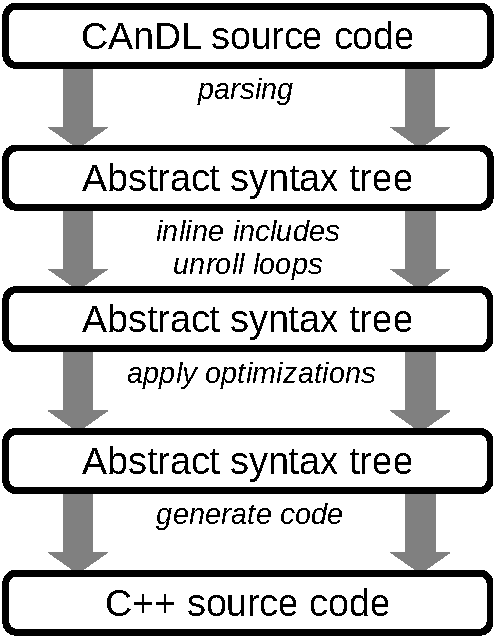
\includegraphics[width=0.85\textwidth]{figures/candlstages.pdf}
\caption{Flow within the CAnDL compiler:
         The CAnDL source code gets lowered in several steps to generated C++
         source code.}
\label{fig:compilerflow}
\end{minipage}
\end{figure}

    The CAnDL compiler is responsible for parsing CAnDL programs and
    generating C++ code from them.
    An overview of its  flow is shown in \Cref{fig:compilerflow}.
    The frontend reads in  CAnDL source code and builds an abstract syntax tree.
    This syntax tree is simplified in two steps to eliminate some of the higher
    order constructs of CAnDL.
    The {\it inheritance} clauses are inlined and contained variables
    transformed accordingly.
    Furthermore, {\it conRange} and {\it disRange} are lowered to
    conjunction and disjunction constructs by duplicating the contained
    constraint code and renaming its variables appropriately for each iteration.
    The remaining core language now consists only of atomics, conjunctions,
    disjunctions and collections.

    The CAnDL compiler then applies a set of optimisations to speed up the
    solving process using the later generated C++ code.
    For example, nested conjunctions and disjunctions are flattened wherever
    possible.
    Furthermore, if shallow equivalence of two variables is enforced in a
    conjunction, one of the two variables is chosen as having higher priority.
    All occurrences of the other variable are then replaced with that one.

    Finally, the compiler generates C++.
    This essentially means generating a function which at runtime constructs
    the constraint problem as a graph structure that is accessible to the
    solver.

\subsubsection{C++ Code Generation}

\begin{figure}[t]
\centering
\begin{lstlisting}[language=CAnDL]
Constraint SimpleAddition
( opcode{addition} = add
∧ {addition}.args[0] = {left}
∧ {addition}.args[1] = {right}) End
\end{lstlisting}
\begin{lstlisting}[language=MyCpp,label={fig:codegen},caption=
   {C++ code generation: The code is generated to first instantiate atomic
    constraints, then compose higher-level constructs and finally assemble a
    backtracking solution for the solver.}]
// Step 1: Instantiate Atomic Constraints
auto constr0 = make_shared<AddInstruction>(model);
auto constr1 = make_shared<FirstArgument> (model);
auto constr2 = make_shared<SecondArgument>(model);
// Step 2: Compose Higher-Level Constraints
auto constr3 = make_shared<Conjunction>(
                   constr0,
                   select<0>(constr1),
                   select<0>(constr2));
// Step 3: Assemble Backtracking Solution
vector<pair<string,shared_ptr<BacktrackingPart>>> result(3);
result[0] = make_pair("addition", constr3);
result[1] = make_pair("left",     select<1>(constr1));
result[2] = make_pair("right",    select<1>(constr2));
\end{lstlisting}
\end{figure}

    The code generation process is demonstrated with an example in
    \Cref{fig:codegen}.
    Every atomic constraint in CAnDL results in a line of C++ code that
    constructs an object of a corresponding class:
    In this case, the three involved atomic constraints are implemented by
    \texttt{AddInstruction}, \texttt{FirstArgument} and \texttt{SecondArgument}.
    These objects are instantiated as shared pointers.

    The compiler then generates analogous objects for the
    \texttt{conjunction}, \texttt{disjunction} and \texttt{collect} structures.
    In our example, this only affects the variable \texttt{addition}, which is
    part of a \texttt{conjunction} clause.
    This results in an additional object construction that instantiates the
    \texttt{Conjunction} class corresponding to the ``$\land$'' operator
    in CAnDL.

    Constraint classes that implement constraints operating on a single
    variable directly expose the \texttt{BacktrackingPart} interface introduced
    in \Cref{cppsolver}.
    In the example, this applies to \texttt{AddInstruction} and
    \texttt{Conjunction}.
    For more complex constraints, the \texttt{select<n>} template is used to
    specify which variable of a constraint is being considered.
    In lines 6--7, this is used to extract the parts of backtracking solutions
    referring to the \texttt{addition} variable, and to then pass them as
    arguments to the conjunction.

    Finally, the generated objects are inserted into a vector, together with the
    corresponding variable names.
    The variables are in the order of appearance in the CAnDL code.
    This vector corresponds to the backtracking solution of the constraint
    problem and is passed to the solver.

\subsection{Developer Tools}

\begin{figure}[t]
\centering
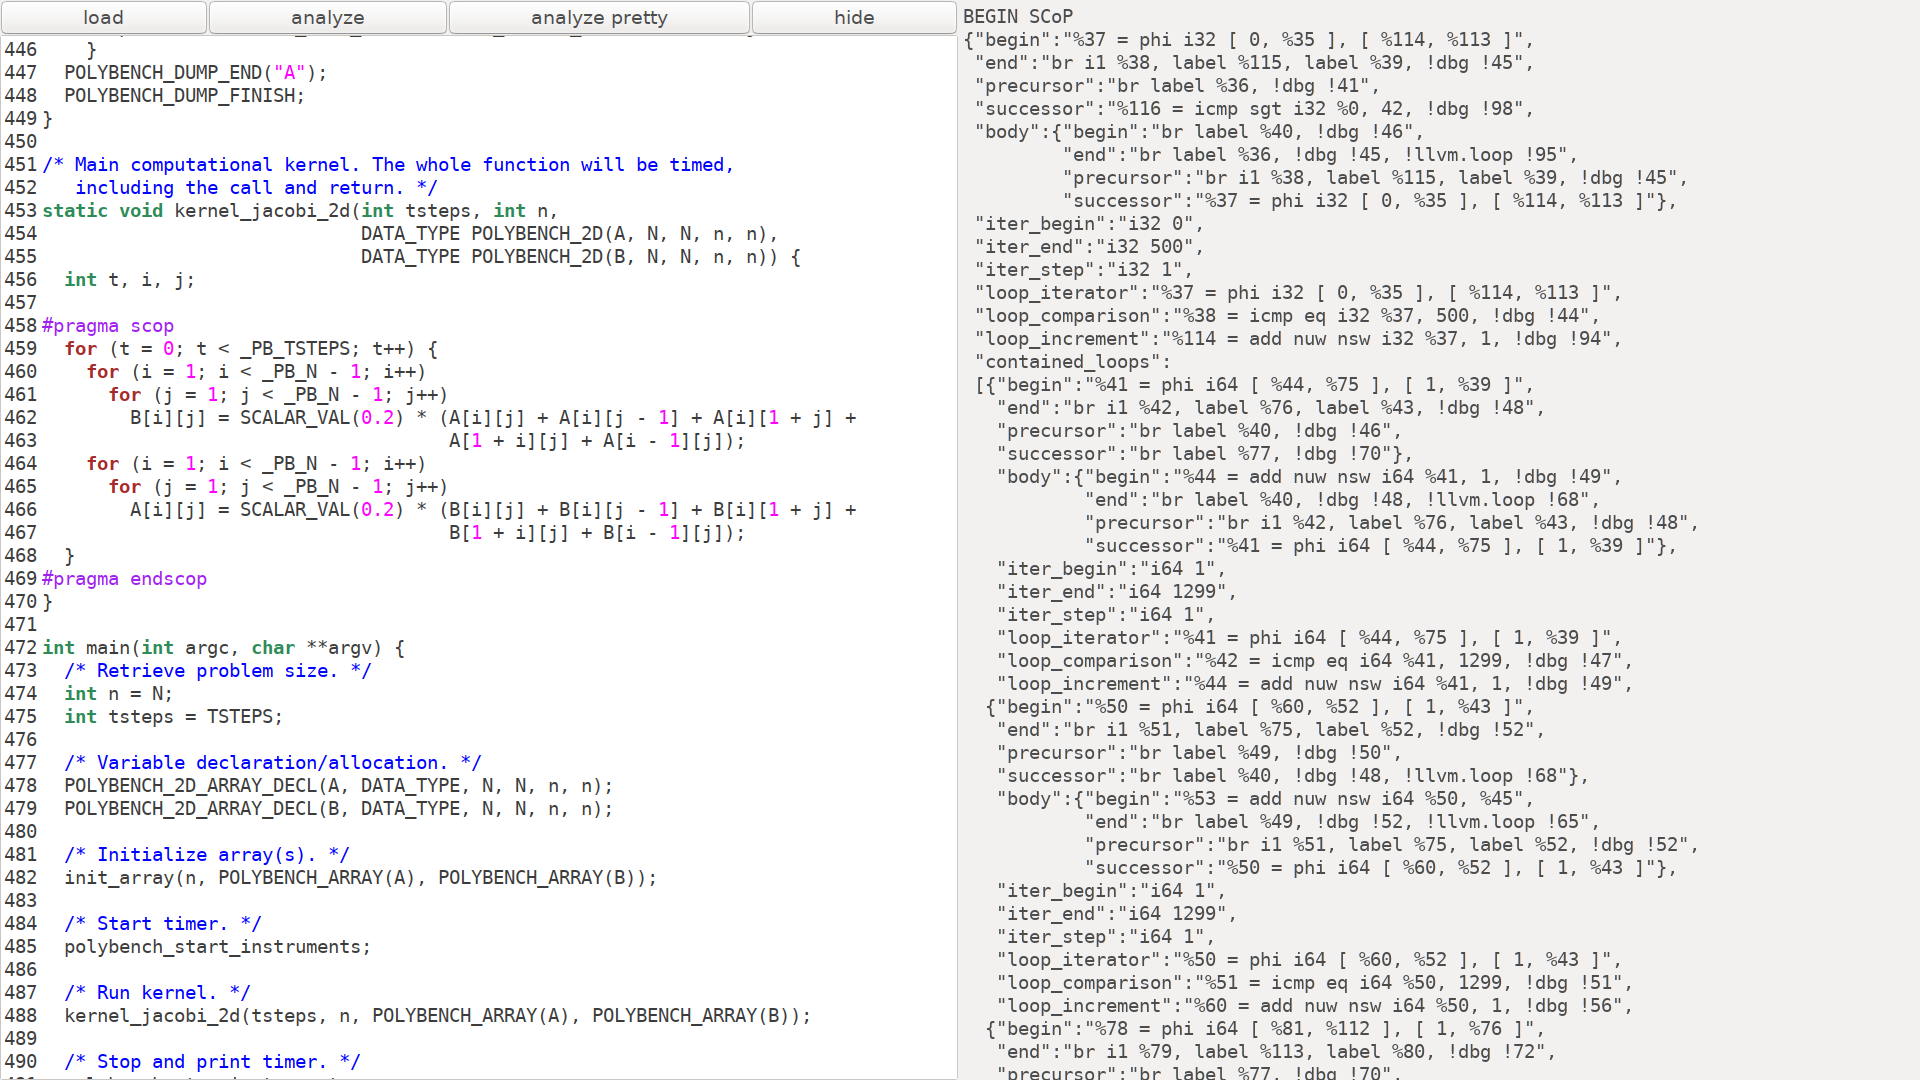
\includegraphics[width=\textwidth]{figures/visual_gui2.png}
\caption{Interactive CAnDL test tool: The left hand panel shows a Static Control
        Part (SCoP) in Polybench jacobi-2d, the right hand panel shows the
        constraint solutions found by the solver.}
\label{fig:gui}
\end{figure}

    CAnDL simplifies the construction of compiler analysis functionality, but
    reasoning about the semantics of compiler intermediate representation
    remains difficult.
    The solver detects whatever the programmer specifies, without any additional
    effort, but it is difficult to ensure that the CAnDL code actually
    specifies the structures that the programmer intended.
    Generally, the accuracy of CAnDL programs can only be ensured with
    thorough testing, and it is important to keep in mind that CAnDL is targeted
    at expert compiler developers.

    In order to make the debugging of CAnDL programs more feasible, 
    supporting tools are provided.
    Most importantly, this includes an interactive GUI, where developers can
    test out corner cases of their CAnDL programs to find false positives and
    false negatives.
    This GUI is shown in \Cref{fig:gui}, with an example from one of the use
    cases presented in \Cref{sec:casestudies}.

    In the left half, part of a C program from the PolyBench benchmark suite
    is visible, which implements a two-dimensional Jacobi stencil.
    The GUI was configured to look for Static Control Parts (SCoPs), as
    described later.
    The user has clicked the ``analyze'' button, which triggered the analysis to
    run by invoking the modified Clang compiler.
    The GUI then read the report file, and printed the results in the right
    hand part of the figure.

    The solver found a SCoP in the IR code (corresponding to lines 459--468 of
    the C program).
    The text on the right shows the hierarchical structure of the solution, with
    IR values assigned to every variable.
    The corresponding C entities can be recovered using the debug
    information that is contained in the generated LLVM IR code.
    By modifying the C code, the developer can now test the detection and
    e.g.\ verify that no SCoP is detected if irregular control flow is
    introduced.

\section{Case Studies}
\label{sec:casestudies}

    The effectiveness of CAnDL was evaluated with three different use cases.
    Firstly, it was used for detecting opportunities to apply a simple peephole
    optimisation.
    Secondly, CAnDL was applied to graphics shader code optimisation.
    Finally, the detection of Static Control Parts (SCoPs) that are
    amenable for polyhedral code transformations was implemented in CAnDL.
    Where possible, the evaluation compares the number of lines of CAnDL code,
    the program coverage achieved and performance against prior approaches.

\subsection{Case Study 1: Simple Optimisations}

\begin{figure}[t]
\begin{lstlisting}[language=CAnDL,label={fig:facopport},caption=
   {Factorisation opportunities in CAnDL: This captures some opportunities that
    LLVM {\tt instcombine} misses. {\tt SumChain} and {\tt MulChain} are
    themselves specified in CAnDL (16 LoC).}]
Constraint ComplexFactorisation
( opcode{value} = add
∧ {sum1.value} = {value}.args[0]
∧ {sum2.value} = {value}.args[1]
∧ include SumChain @ {sum1}
∧ {product1.value} = {sum1.last_factor}
∧ include MulChain @ {product1}
∧ {product1.last_factor} = {product2.last_factor}
∧ include SumChain @ {sum2}
∧ {product2.value} = {sum2.last_factor}
∧ include MulChain @ {product2}) End
\end{lstlisting}
\end{figure}

    Arithmetic simplifications in LLVM are implemented in the
    \texttt{instcombine} pass.
    One example of this is the standard factorisation optimisation that uses the
    law of distributivity to simplify integer calculations as shown in
    \Cref{fig:factorization1}.
    Within {\tt instcombine}, this is implemented in 203 lines of code, and
    furthermore uses supporting functionality that is shared with other peephole
    optimisations.
    \begin{align}
        a*b+a*c\rightarrow a*(b+c)
        \label{fig:factorization1}
    \end{align}

    This analysis problem can be formulated in CAnDL as shown in
    \Cref{fig:facopport}.
    Crucially, at lines 5,7,9,11, the specification makes use of
    \texttt{SumChain} and \texttt{MulChain}, which allows the CAnDL program
    to capture a large, generalised class of opportunities for factorisation.
    The \texttt{instcombine} pass has limited support for this, and
    first requires the application of associative and commutative laws to
    reorder the values.
    For example, this is needed for \Cref{fig:factorization2}, and only
    partially supported by LLVM with the additional \texttt{reassociate} pass.
    \begin{align}
        a*b+c+d*a*e->a*(b+d*e)+c
        \label{fig:factorization2}
    \end{align}

\subsubsection{Experimental Setup}

    The specification in \Cref{fig:facopport} was evaluated against the default
    factorisation optimisation in \texttt{instcombine} on three different
    benchmark collections:
    The sequential C versions of the NAS Parallel Benchmarks
    \citep{Bailey1991NPB}, as provided by \citet{seo2011performance};
    the C/C++ Parboil benchmarks from \citet{stratton2012parboil};
    and the OpenMP C/C++ programs of the Rodinia benchmark suite
    \citep{Che2009Rodinia}.
    The existing LLVM \texttt{instcombine} pass was extended, so that it
    automatically reports every time that it successfully applies the
    \texttt{tryFactorization} function.  

    % NPB:     29047 loc
    % Parboil:  7358 loc
    % Rodinia: 58510 loc
    The individual benchmark programs in the three benchmark
    suites consist of 94915 lines of code in total.
    For each benchmark suite, the total number of reported factorisations as
    well as the total compilation time were measured.
    The standard LLVM optimisation was then disabled, and the CAnDL-generated
    detection functionality was used.
    The same application programs were compiled with the same version of Clang
    and identical compiler options, reporting the number of factorisations
    found, and again measuring the total compilation time.
    This timing includes all the other passes within LLVM, plus the CAnDL code
    path.

\subsubsection{Results}

\begin{table}[t]
  \centering
  \definecolor{tableShade}{gray}{0.9}
  \rowcolors{1}{}{tableShade}
  \begin{tabular}{lll}
    \toprule
    & {\bf LLVM} & {\bf CAnDL} \\
    \midrule
    Lines of Code & 203 & 12 \\
    Detected in NPB & 1 & 1 + 2 \\
    Detected in Parboil & 0 & 0 + 1\\
    Detected in Rodinia & 24 & 24 + 4\\
    Total Compilation time & 152.2s & 152.2s+7.8s \\
    \bottomrule
\end{tabular}
\caption{Factorisations enabled by LLVM vs CAnDL}
\label{fig:factorization_results}
\end{table}

    The results of the evaluation are shown in
    \Cref{fig:factorization_results}.
    In two of the benchmark collections -- NPB and Parboil -- there are
    only a limited number of factorisation opportunities.
    LLVM was unable to perform any factorisation in the entire Parboil suite.
    However, the Rodinia suite contains more opportunities, mostly in the
    Particlefilter and Mummergpu programs.

    In all three benchmarks suites, the CAnDL system found all the factorisation
    opportunities that the \texttt{instcombine} pass identified.
    In addition, it detected an additional 7 cases across all programs.
    Just 12 lines of CAnDL code were able to capture more factorisation
    opportunities than 200 lines of C++ code in LLVM.

    Using CAnDL on large benchmark suites only increased total compilation time
    by ${\sim}5\%$.
    Given the generally small impact of individual peephole optimisations, an
    evaluation of the performance or code size impact vs {\tt instcombine} is
    unlikely to yield significant results.

\subsection{Case Study 2: Graphics Shader Optimisations}

\begin{figure}[t]
\begin{lstlisting}[language=CAnDL,label={fig:Lewis},caption=
   {CAnDL defines multiplication chains with genuine vectors and hoisted
    scalars:
    After separating the two cases, some of the multiplications can be performed
    on scalars instead.}]
Constraint FloatingPointAssociativeReorder
( include VectorMulChain
∧ collect j N
∧ ( {hoisted[k]} = {factors[i]} forany i=0..N
  ∧ include ScalarHoist({hoisted[j]}->{out},
                       {scalar[j]}->{in})@{hoist[j]})
∧ collect j N
  ( {nonhoisted[j]}  = {factors[i]} forany  i=0..N
  ∧ {nonhoisted[j]} != {hoisted[i]} foreach i=0..N))
End
\end{lstlisting}
\end{figure}

    Graphics computations often involve arithmetic on vectors of
    single-precision floating-point values, which can represent vertex positions
    in space or colour values.
    Established graphics shader compilers utilise the LLVM intermediate
    representation internally \citep{cudacompiler}.

    In real shader code, there are often element-wise products of several
    floating-point vectors, where some of the factors are actually scalars
    that were hoisted to vectors.
    By reordering the factors and delaying the hoisting to vectors, some of the
    element-wise vector products can be simplified to products on scalars, as
    shown by example in the following equation.
    \begin{align*}
        \vec x={}&\vec a*_v\vec b*_v\text{vec3}(c)*_v\vec d*_v\text{vec3}(e)\\
        ={}&\text{vec3}(c*e)*\vec a*_v\vec b*_v\vec d
    \end{align*}

    For general purpose code, such reordering can be problematic.
    This is due to computation artefacts in floating-point arithmetic.
    However, this is generally no problem in the domain of graphics processing.
    Instead, associative reordering can result in performance improvements
    when combined with lowering to scalar multiplications as discussed above.

    The required analysis functionality for this optimisation was implemented
    with CAnDL, as shown in \Cref{fig:Lewis}.
    Firstly, the specification includes \texttt{VectorMulChain} to detect 
    chains of floating point vector multiplications.
    In lines 4--6, all the factors that are hoisted from some scalar are
    collected into the array {\tt hoisted}.
    Correspondingly, all the other factors are collected into the array
    {\tt nonhoisted} at lines 7--9.

    {\tt VectorMulChain} and {\tt ScalarHoist} are themselves implemented as
    CAnDL programs.
    {\tt VectorMulChain} discovers chains of floating point vector
    multiplications in the IR code.
    It is defined very similarly to {\tt SumChain} and {\tt MulChain}, which
    were used in the previous case study.
    It guarantees chains of maximal length by checking that neither of the first
    two factors is a multiplication itself, and that the last factor is not used
    in any multiplication.

    \texttt{ScalarHoist} operates on the variables {\tt in} and {\tt out}, as
    well as some internals.
    It specifies that {\tt out} is a vector generated from {\tt in} by setting
    all vector dimensions to the value of {\tt in}.
    The implementation of this is very specific to LLVM and involves
    combinations of the LLVM IR instruction {\tt insertelement} and
    {\tt shufflevector}

\subsubsection{Experimental Setup}

    The LunarGLASS project \citep{lunarglass} was used in this work to
    transform shaders into LLVM IR and back after optimisation.
    The CAnDL specification was applied to all fragment shaders in the
    GFXBench 4.0 suite from \citet{gfxbench}.
    A corresponding transformation pass was added to LLVM, which uses the
    detected solutions to implement the described optimisation.
    This is done by constructing the appropriate scalar and vector
    multiplications from the arrays {\tt hoisted} and {\tt nonhoisted}, and then
    replacing the result of the original vector multiplication chain with the
    final multiplication in these newly generated instructions.
    Standard dead code elimination automatically removes the remnants of the
    original calculation.

    The performance impact was evaluated on the Qualcomm Adreno 530 GPU.
    To measure the baseline of benchmark performance, all shaders were
    compiled with the default Qualcomm graphics stack.
    They were then compiled with LunarGLASS into LLVM, CAnDL was applied, and
    they were transformed back into GLSL code \citep{Rost:2009:OSL:1696393}.
    To evaluate the impact, the result was again passed through the default
    graphics stack and the performance of the shaders measured.

\subsubsection{Results}

\begin{figure}[t]
\centering
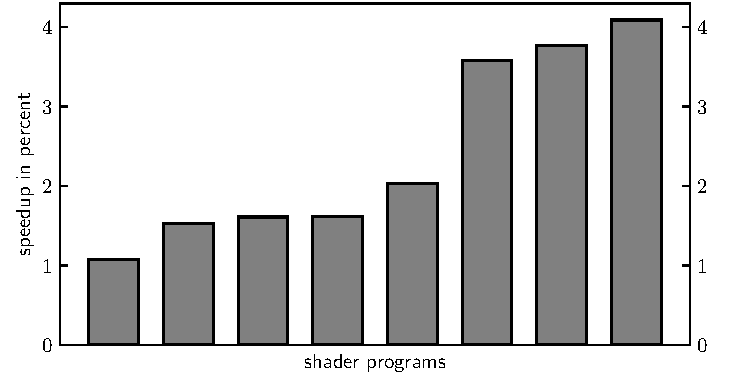
\includegraphics[width=0.66\linewidth]{figures/qualcomm_plot.pdf}
\caption{Speedup on Qualcomm Adreno 530 (evaluated on HTC 10, running Android 7.0)
         \leftskip=0pt\rightskip=0pt}
\label{fig:qualcommspeedup}
\end{figure}

%\begin{figure}[b]
%\centering
%\begin{tabular}{|l||l|l|}
%\hline
%         & LLVM  &CAnDL \\
%\hline
%\hline
%Lines of Code & Not implemented& 10 \\ \hline
%Detected in GFX 4.0 & - & 19 \\ \hline
%\hline
%\end{tabular}
%\caption{Shader optimization LLVM vs CAnDL}
%\label{fig:candlshader}
%\end{figure}

    There were 19 solutions to the specification across the benchmarks, and
    the transformation had an impact on the performance of 8 fragment shaders.
    The resulting performance impact is shown in \Cref{fig:qualcommspeedup}.
    Evidently, there are opportunities for such associative reordering that
    the default graphics stack misses.
    Although the performance impact was moderate with 1--4\% speedup on 8
    of the fragment shaders, it shows how new analysis can be rapidly prototyped
    and evaluated with only a few lines of code.

\subsection{Case Study 3: Detection of Polyhedral SCoPs}

    The polyhedral model
    \citep{Karp:1967:OCU:321406.321418,benabderrahmane2010polyhedral} allows
    compilers to utilise powerful mathematical reasoning to detect parallelism
    opportunities in sequential code and to implement code transformations.
    However, this applies only for a restrictive class of well-structured loop
    nests.
    More precisely, conventional polyhedral code transformations are applicable
    to Static Control Parts (SCoPs).
    Detecting SCoPs is a fundamental and necessary first step for any later
    polyhedral optimisation.

    Implementations of the polyhedral model may differ in their precise
    definition of SCoPs.
    The definition of Semantic SCoPs from the Polly compiler by
    \citet{Lengauer2012Polly} was used for reference here.
    SCoP detection functionality was implemented in CAnDL and compared against
    Polly, which is also implemented as an extension to LLVM.
    The use of the same definition for SCoPS and the implementation in the same
    compiler infrastructure allow for a direct comparison between Polly and
    CAnDL.
    The specification of SCoPs is significantly more complex than the required
    CAnDL code for the previous case studies.
    However, it can be broken into several components, with some of them shown
    in \Cref{polyhedralCAnDL}
    \footnote{The complete CAnDL code for this section is in
    Appendix~\ref{appendix:CAnDLpoly}.}.

    \paragraph*{Structured Control Flow}
    SCoPs require well-structured control flow.
    This means that each conditional jump within the
    corresponding piece of LLVM IR is accounted for by for-loops and
    conditionals.
    This is ensured with the \texttt{collect} statement, as in
    \Cref{fig:collectexample}.
    The construct is used with the CAnDL specifications \texttt{ForLoop} and
    \texttt{Conditional} that describe the control flow of for-loops and
    conditionals.
    All the involved conditional jump instructions are extracted, and  another
    \texttt{collect} is then used to verify that these are indeed all
    conditional jumps within the potential SCoP.

    Once the control flow has been established, the iterators that are
    involved in the loops are used to define affine integer computations in the
    loop.
    This is done in a brute-force fashion with a recursive constraint program.
    It is then checked that the iteration domain of all the for-loops is
    well-behaved, i.e.\ the boundaries are affine in the loop iterators.

    \paragraph*{Affine Memory Access}
    All memory accesses in the SCoP must be affine.
    For this to be true, it needs to be verified that for each {\tt load} and
    {\tt store} instruction, the base pointer is loop invariant and the index is
    calculated affinely.
    The loop invariant base pointer is easily guaranteed using the
    \texttt{LocalConst} program from \Cref{localconstant}.

    Checking the index calculations is more involved and is again based on the
    {\tt collect} method that was demonstrated in \Cref{fig:collectexample}.
    The {\tt collect} construct is used to find all of the affine memory
    accesses in all the loop nests.
    Then another {\tt collect} gathers all \texttt{load} and \texttt{store}
    instructions, and it is verified that both collections are identical.

\begin{figure}[p]
\lstset {
 basicstyle=\linespread{0.915}\small\ttfamily
}
\begin{lstlisting}[language=CAnDL, label=polyhedralCAnDL, caption=
   {Fragments from the specification of Scalar Control Parts (SCoPs) in CAnDL:
    SCoPs are defined at lines 1--11 by applying multiple restrictions to the
    containing loop.
    These restrictions are then individually implemented in CAnDL, including
    {\tt StructuredControlFlow} and {\tt AffineMemAccesses}, shown in
    lines 13--33 and lines 35--54 respectively
    (cf.\ Appendix \ref{appendix:CAnDLpoly}).}]
Constraint SCoP
( include For @ {loop}
∧ include StructuredControlFlow({loop}->{scope}) @ {control}
∧ {inputs[0]} = {loop.iterator}
∧ {inputs[i]} = {control.loop[i-1].iterator} foreach i=1..10
∧ include AffineControlFlow({loop}->{scope},
                          {inputs}->{inputs}) @ {control}
∧ include AffineMemAccesses({loop}->{scope},
                          {inputs}->{inputs}) @ {accesses}
∧ include SideEffectFreeCalls({loop}->{scope}) @ {effects})
End

Constraint StructuredControlFlow
( collect i 20 ( opcode{branch[i].value} = branch
               ∧ {branch[i].target1} =
                     {branch[i].value}.successors[0]
               ∧ {branch[i].target2} =
                     {branch[i].value}.successors[1]
               ∧ include ScopeValue({scope}->{scope},
                          {branch[i].value}->{value}))
∧ collect i 10 ( include For @ {loop[i]}
               ∧ domination({scope.begin},
                          {loop[i].begin})
               ∧ strict_post_domination({scope.end},
                                      {loop[i].end}))
∧ collect i  10 ( include IfBlock @ {ifblock[i]}
               ∧ domination({scope.begin},
                       {ifblock[i].precursor})
               ∧ strict_post_domination({scope.end},
                                   {ifblock[i].successor}))
∧ {loop[0..10].end,ifblock[0..10].precursor}
      is the same set as {branch[0..20].value})
End

Constraint AffineMemAccesses
( collect x 20 ( include MemoryAccess({scope}->{scope})
                                      @ {newaccess[x]}
               ∧ opcode{newaccess[x].pointer} = gep
               ∧ domination({scope.begin},
                     {newaccess[x].pointer})
               ∧ {newaffine[x].value} =
                     {newaccess[x].pointer}.args[1])
∧ collect x 20 ( include MemoryAccess({scope}->{scope})
                                      @ {newaccess[x]}
               ∧ opcode{newaccess[x].pointer} = gep
               ∧ domination({scope.begin},
                     {newaccess[x].pointer})
               ∧ {newaffine[x].value} =
                     {newaccess[x].pointer}.args[1]
               ∧ include AffineCalc[M=10,N=6](
                                          {scope}->{scope},
                                         {inputs}->{input})
                                          @ {newaffine[x]}))
End
\end{lstlisting}
\end{figure}

\subsubsection{Experimental Setup}

    The reliable detection of SCoPs was evaluated on the PolyBench suite by
    \citet{polybench}, a collection of 31 benchmarks containing SCoPs of
    differing complexity from several application domains.
    For both the CAnDL-based approach and for the evaluation of Polly, it was
    counted how many of the computational kernels contained in the benchmark
    suite were captured in their entirety by the respective analysis.

    Some post-processing of the generated constraint solutions was required to
    compare the results of CAnDL and Polly.
    This is because the CAnDL results are not in the JSCoP format that Polly
    generates, but contain instead the raw constraint solution represented
    as a JSON file.
    Additionally, the CAnDL implementation does not merge consecutive
    outer level loops into a single SCoP of maximum size.
    Therefore, the detected loops from the CAnDL solver were extracted and
    grouped together.
    A Python script was then used to verify that they precisely covered the
    SCoPs detected by Polly.

\subsubsection{Results}

    \Cref{fig:candlvspolly} shows that the CAnDL specification captured all the
    SCoPs that Polly detected.
    To measure the lines of code required, the CAnDL version was compared with
    the amount of code in \texttt{ScopDetection.cpp} of Polly.
    The same detection results were achieved with much fewer lines of code in
    CAnDL.
    Detecting SCoPs with CAnDL took under one second for each program in
    PolyBench.
    Note that the line count that is given for the CAnDL program does not
    include all the CAnDL code involved in the detection of polyhedral regions.
    Code that is not specific to this idiom (such as loop structures) is
    considered as part of the CAnDL standard library.
    In the same way, the line count for Polly does not account for additional
    code that Polly relies on when detecting SCoPS, e.g.\ the expansive
    ScalarEvolution pass.

    With a high-level representation of SCoPs, CAnDL allows polyhedral
    compiler researchers to explore the impact of relaxing or tightening the
    exact definition of SCoPs in a straightforward manner, enabling rapid
    prototyping.
    Simple commenting out of constraint statements in the CAnDL specification
    relaxes the conditions.

\begin{table}[ht]
    \centering
\begin{tabular}{|l||l|l|}
\hline
         & Polly & CAnDL \\
\hline
\hline
Lines of Code & 1903 & 45 \\ \hline
Detected in datamining & 2 & 2\\
Detected in Linear-algebra & 19 & 19\\
Detected in medley & 3 & 3\\
Detected in stencils & 6 & 6\\ \hline
%Compilation time & 24.4s+37.5s & 24.4s+12.7s \\ \hline
\end{tabular}
    \caption{SCoPs detected Polly vs CAnDL}
    \label{fig:candlvspolly}
\end{table}

\section{Conclusions}

    Optimising compilers require sophisticated program analysis in order to
    generate performant code.
    The state-of-the-art approach for implementing this functionality manually
    in C++ is not satisfactory, as exemplified by the complicated and
    error-prone {\tt instcombine} pass in the LLVM compiler infrastructure.

    The domain-specific Compiler Analysis Description Language (CAnDL) provides
    a more efficient approach.
    CAnDL specifications can automatically generate compiler analysis
    passes from a declarative description.
    They are easier to program, and significantly reduce the code size and
    complexity when comparing against manual C++ implementations.
    Although CAnDL is based on a constraint programming paradigm and uses a
    backtracking solver to analyse LLVM IR code, it results in only moderate
    compile time increases.

    Many compiler analysis tasks are suitable for implementation with CAnDL.
    It can be used for the detection of standard peephole optimisation
    opportunities and the rapid prototyping of graphics shader optimisations.
    Despite its general approach, CAnDL scales to complex domain-specific code
    structures and can efficiently recognise large code regions suitable for
    polyhedral transformations.

    \paragraph*{Outlook}
    The third case study showed that CAnDL can express the algorithmic structure
    of complex loop nests, not just peephole optimisation opportunities.
    This enables the capturing of entire loops at a time.
    The following chapters expand on this observation by investigating how the
    recognition of computational idioms in loops can be leveraged for
    performance.
    Where SCoPs were reported without informing additional compiler
    transformations, \Cref{chapter:reductions} applies auto-parallelisation
    techniques to a broad generalisation of reduction computations.
    
    